\subsection{Pooling} \label{subs:pooling}
Pooling layers are inserted between successive convolutional layer. It aims at reducing the spatial size of each \acrshort{fm}. It reduces the number of parameters and the computation of the network while also increasing the receptive field \cite{shawahna_fpga-based_2019}. The layer divides each \acrshort{fm} in regions of size $K \title K$ and outputs one pixel from each region. This way, we can keep the number of channel and reduce each spatial dimension by $K$.

Various pooling functions can be used, but the most common form is with filters of size $2 \times 2$ where the MAX or AVG operation selects the highest pixel from 4 samples (meaning a reducion 75\%) \cite{suda_throughput-optimized_2016}. An illustration can be found in figure \ref{fig:pool}.
%
\begin{figure}
    \centering
    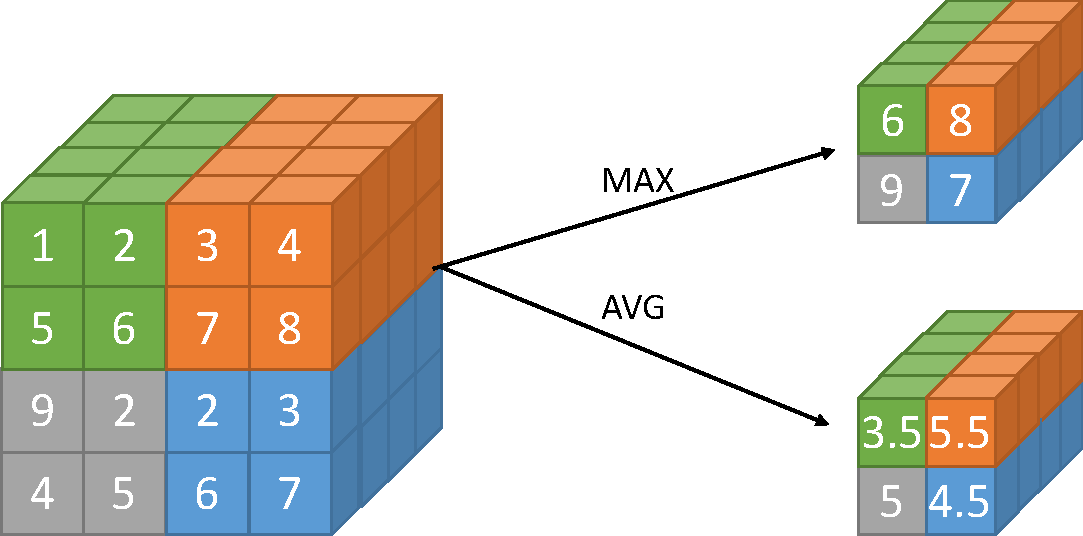
\includegraphics[width=\textwidth]{pooling.pdf}
    \caption{An example of pooling layers}
    \label{fig:pool}
\end{figure}
